\documentclass[landscape,a0paper,fontscale=0.292]{baposter}

\usepackage[vlined]{algorithm2e}
\usepackage{times}
\usepackage{calc}
\usepackage{url}
\usepackage{graphicx}
\usepackage{amsmath}
\usepackage{amssymb}
\usepackage{relsize}
\usepackage{multirow}
\usepackage{booktabs}

\usepackage{graphicx}
\usepackage{multicol}
\usepackage[T1]{fontenc}
\usepackage{ae}
\usepackage{enumitem}
\setlist[itemize]{nosep}

\usepackage{colortbl}
\usepackage{xcolor}
\usepackage{setspace}

\usepackage{comment}
%\usepackage{gensymb} % for \degree
\graphicspath{{images/}}

\setlist[itemize]{leftmargin=*,nosep}
    \setlength{\columnsep}{0.7em}
    \setlength{\columnseprule}{0mm}

\setlist[enumerate]{leftmargin=2.5em,nosep}
    \setlength{\columnsep}{1.0em}
    \setlength{\columnseprule}{0mm}

% %%%%%%%%%%%%%%%%%%%%%%%%%%%%%%%%%%%%%%%%%%%%%%%%%%%%%%%%%%%%%%%%%%%%%%%%%%%%%%%%
% % Save space in lists. Use this after the opening of the list
% %%%%%%%%%%%%%%%%%%%%%%%%%%%%%%%%%%%%%%%%%%%%%%%%%%%%%%%%%%%%%%%%%%%%%%%%%%%%%%%%
% \newcommand{\compresslist}{%
% \setlength{\itemsep}{0pt}%
% \setlength{\itemsep}{0pt}%
% \setlength{\parskip}{0pt}%
% \setlength{\parsep}{0pt}%
% }
\renewcommand{\rmdefault}{ptm} % Arial
\renewcommand{\sfdefault}{ptm} % Arial
\definecolor{purpleheart}{rgb}{0.41, 0.21, 0.61}
\definecolor{purple(html/css)}{rgb}{0.5, 0.0, 0.5}
\newcommand{\headercolor}{white}
\newcommand{\subheadercolor}{black}

%% Network names
\newcommand{\RefineStage}{RefineNet\xspace}
\newcommand{\CoarseStage}{CoarseNet\xspace}
\newcommand{\CoarseStagenospace}{CoarseNet}
\newcommand{\Weightnetwork}{Weight network\xspace}
\newcommand{\weightnetwork}{weight network\xspace}
\newcommand{\Flownetwork}{Flow network\xspace}
\newcommand{\flownetwork}{flow network\xspace}
\newcommand{\featurealignmodule}{deformable alignment module\xspace}
\newcommand{\featurefusionmodule}{temporal attention fusion module\xspace}
\newcommand{\expolowthr}{0.15}
\newcommand{\expohighthr}{0.9}
\newcommand{\SingleStageRefineStage}{RefineNet$^\dag$\xspace}

%% Exposure description
\newcommand{\twoexposure}{two-exposure\xspace}
\newcommand{\threeexposure}{three-exposure\xspace}
\newcommand{\ntwoExposure}{2-Exposure\xspace}
\newcommand{\nthreeExposure}{3-Exposure\xspace}
\newcommand{\lowexposure}{low-exposure\xspace}
\newcommand{\middleexposure}{middle-exposure\xspace}
\newcommand{\highexposure}{high-exposure\xspace}
\newcommand{\LowExposure}{Low-Exposure\xspace}
\newcommand{\MiddleExposure}{Middle-Exposure\xspace}
\newcommand{\HighExposure}{High-Exposure\xspace}
\newcommand{\AllExposure}{All-Exposure\xspace}

\newcommand{\lineardomain}{linear radiance domain\xspace}

% Metrics
\newcommand{\PSNRL}{PSNR-L\xspace}
\newcommand{\PSNRT}{PSNR\xspace}
\newcommand{\SSIMT}{SSIM-T\xspace}
\newcommand{\VQM}{HDR-VQM\xspace}
\newcommand{\VDP}{HDR-VDP2\xspace}

% Mathematical variables
\newcommand{\crf}{\mathcal{F}}
\newcommand{\hdr}{H}
\newcommand{\tmhdr}{T}
\newcommand{\gttmhdr}{\tilde{\tmhdr}}
\newcommand{\ldr}{L}
\newcommand{\lhdr}{I}
\newcommand{\originldr}{\tilde{\ldr}}
%\newcommand{\hdrtoldr}{l}
\newcommand{\ldrtohdr}{h}
\newcommand{\hdrtoldr}{g}
\newcommand{\expt}{t}
\newcommand{\flow}{F}
\newcommand{\warpldr}{\hat{L}}
\newcommand{\warplhdr}{\hat{I}}
\newcommand{\weight}{\omega}
\newcommand{\coarsehdr}{\hdr^c}
\newcommand{\coarsetmhdr}{\tmhdr^c}
\newcommand{\coarseloss}{\mathcal{L}^\text{c}}
\newcommand{\refinehdr}{\hdr^r}
\newcommand{\refinetmhdr}{\tmhdr^r}
\newcommand{\finalhdr}{\hdr}
\newcommand{\finaltmhdr}{\tmhdr}
\newcommand{\refineloss}{\mathcal{L}^r}
\newcommand{\totalloss}{\mathcal{L}}
\newcommand{\validmask}{M}
\newcommand{\feature}{F}
\newcommand{\alignedfeature}{\tilde{F}}

% Datasets
\newcommand{\staticdatalong}{\emph{static scenes with GT}\xspace}
\newcommand{\staticdataWithMotion}{\emph{static scenes} augmented with random global motion\xspace}
\newcommand{\dynamicgtdatalong}{\emph{dynamic scenes with GT}\xspace}
\newcommand{\dynamicdatalong}{\emph{dynamic scenes without GT}\xspace}
\newcommand{\staticdata}{$\mathcal{D}_s^{gt}$\xspace}
\newcommand{\dynamicgtdata}{$\mathcal{D}_d^{gt}$\xspace}
\newcommand{\dynamicdata}{$\mathcal{D}_d$\xspace}
\newcommand{\kalantaridata}{\emph{Kalantari13} dataset\xspace}
\newcommand{\traindataHDR}{$D_\text{HDR}$\xspace}
\newcommand{\traindataVimeo}{$D_\text{Vimeo}$\xspace}

\newcommand{\NumOfStaticTwoExp}{49}
\newcommand{\NumOfStaticThreeExp}{48}
\newcommand{\NumOfDynamicGTTwoExp}{76}
\newcommand{\NumOfDynamicGTThreeExp}{108}
\newcommand{\NumOfDynamicTwoExp}{37}
\newcommand{\NumOfDynamicThreeExp}{38}

\newcommand{\pokerscene}{\scene{Poker Fullshot}}
\newcommand{\carouselscene}{\scene{Carousel Fireworks}}
\newcommand{\ThrowTowelScene}{\scene{Throwing Towel 2Exp}}
\newcommand{\NinjaScene}{\scene{Ninja 2Exp}}
\newcommand{\FireScene}{\scene{Fire 2Exp}}
\newcommand{\CleaningScene}{\scene{Cleanining 3Exp}}
\newcommand{\DogScene}{\scene{Dog 3Exp}}
\newcommand{\EmailScene}{\scene{Checking Email 3Exp}}

% Methods
\newcommand{\YanCVPR}{Yan19~\cite{yan2019attention}\xspace}
\newcommand{\KalantariTOG}{Kalantari13~\cite{kalantari2013patch}\xspace}
\newcommand{\KalantariEG}{Kalantari19~\cite{kalantari2019deep}\xspace}

\DeclareMathOperator*{\Sign}{Sign} 
\DeclareMathOperator*{\XNOR}{XNOR} 
\DeclareMathOperator*{\NOTs}{NOT}
\DeclareMathOperator*{\Popcount}{Popcount}

\DeclareMathOperator*{\argmin}{argmin} 
\DeclareMathOperator*{\inputs}{input}
\DeclareMathOperator*{\w}{w}


\definecolor{bordercol}{RGB}{40,40,40}
\definecolor{headercol1}{RGB}{186,215,230}
\definecolor{headercol2}{RGB}{80,80,80}
\definecolor{headerfontcol}{RGB}{0,0,0}
\definecolor{boxcolor}{RGB}{186,215,230}
%%%%%%%%%%%%%%%%%%%%%%%%%%%%%%%%%%%%%%%%%%%%%%%%%%%%%%%%%%%%%%%%%%%%%%%%%%%%%
%% Begin of Document
%%%%%%%%%%%%%%%%%%%%%%%%%%%%%%%%%%%%%%%%%%%%%%%%%%%%%%%%%%%%%%%%%%%%%%%%%%%%%
\begin{document}
%%%%%%%%%%%%%%%%%%%%%%%%%%%%%%%%%%%%%%%%%%%%%%%%%%%%%%%%%%%%%%%%%%%%%%%%%%%%%
%% Here starts the poster
%%---------------------------------------------------------------------------
%% Format it to your taste with the options
%%%%%%%%%%%%%%%%%%%%%%%%%%%%%%%%%%%%%%%%%%%%%%%%%%%%%%%%%%%%%%%%%%%%%%%%%%%%%
\begin{poster}{
    % Show grid to help with alignment
    grid=false,
    columns=6,
    % Column spacing
    colspacing=0.7em,
    % Color style
    headerColorOne=purple(html/css),
    borderColor=purple(html/css),
    %headerColorOne=purpleheart,
    %borderColor=purpleheart,
    %headerColorOne=cyan!20!white!90!black,
    %borderColor=cyan!30!white!90!black,
    % Format of textbox
    textborder=faded,
    % Format of text header
    headerborder=open,
    headershape=roundedright,
    headershade=plain,
    background=none,
    bgColorOne=cyan!50!white,
    headerheight=0.12\textheight
}
% Eye Catcher
{
	%\begin{tabular}{c}
        \raisebox{0.6\height}{
\includegraphics[height=0.05\linewidth]{logo/KHU_logo}}\\
    %\end{tabular}
    %\makebox[0.005\textwidth]{} 
    %\raisebox{0.00\height}{\includegraphics[height=0.045\linewidth]{logo/alibaba.png}}
    %\makebox[0.005\textwidth]{} 
    %\raisebox{0.00\height}{\includegraphics[height=0.045\linewidth]{logo/PolyU.svg.png}}
}
% Title
{
    \sc\Large\bf MST-compression: Compressing and Accelerating Binary Neural Networks with Minimum Spanning Tree
}
% Authors
{
    {\large Quang Hieu Vo \quad Linh-Tam Tran \quad Sung-Ho Bae \quad Lok-Won Kim \quad Choong Seon Hong} \\
    {{\normalsize Department of Computer Science and Engineering, Kyung Hee University, South Korea}}
}
% University logo
{
    \begin{tabular}{c}
        \raisebox{-1.0\height}{
\includegraphics[width=0.15\linewidth]{logo/ICCV23_logo.png}}\\
        %\raisebox{-0.7\height}{\includegraphics[width=0.15\linewidth]{images/qrcode.pdf}}
    \end{tabular}
}

%%%%%%%%%%%%%%%%%%%%%%%%%%%%%%%%%%%%%%%%%%%%%%%%%%%%%%%%%%%%%%%%%%%%%%%%%%%%%%
%%% Now define the boxes that make up the poster
%%%---------------------------------------------------------------------------
%%% Each box has a name and can be placed absolutely or relatively.
%%% The only inconvenience is that you can only specify a relative position 
%%% towards an already declared box. So if you have a box attached to the 
%%% bottom, one to the top and a third one which should be inbetween, you 
%%% have to specify the top and bottom boxes before you specify the middle 
%%% box.
%%%%%%%%%%%%%%%%%%%%%%%%%%%%%%%%%%%%%%%%%%%%%%%%%%%%%%%%%%%%%%%%%%%%%%%%%%%%%%

%%%%%%%%%%%%%%%%%%%%%%%%%%%%%%%%%%%%%%%%%%%%%%%%%%%%%%%%%%%%%%%%%%%%%%%%%%%%%%
\headerbox{\bf\color{\headercolor} Contribution}{name=contribution,column=0,row=0,span=1}{
    %\begin{minipage}[c]{0.48\linewidth}
        \textbf{\color{\subheadercolor}Motivation:} Propose a comprehensive method from training to HW implementation to compress Binary Neural Networks (BNNs) inference with high throughput via reordering the output calculation for convolution and fully connected layers.
        
    %\end{minipage}
    %\hfill
    \textbf{\color{\subheadercolor}Key contributions:}
    \begin{itemize}
    	\item Analyze the role of Minimum Spanning Tree (MST) to reorder output calculation in BNNs.
    	\item An algorithm toward reducing MST distance right at training phase, leading to inference computation reduction.	
    	\item A supportive hardware accelerator for MST compression method. 
    \end{itemize}  

    
}

\headerbox{\bf\color{\headercolor} MST-compression for Inference BNN Acceleration}{name=abstract,column=0,below=contribution,span=4}{

\begin{minipage}[t]{0.33\linewidth}
	\textbf{\color{\subheadercolor}MST exploration for a conv computation order}
		%\vspace{-0.5em}
	    \begin{center}
	        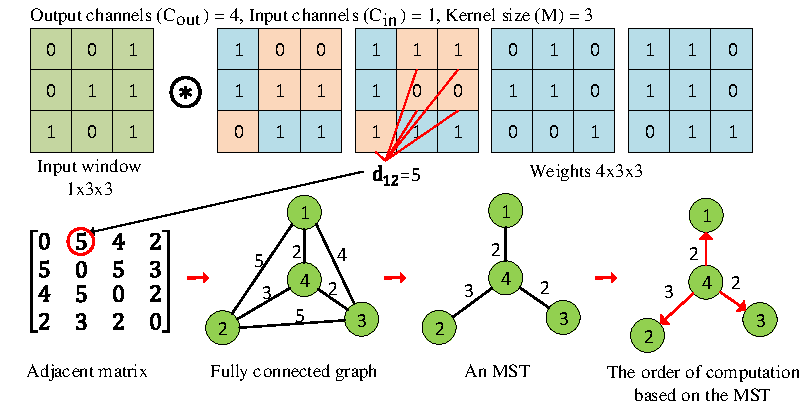
\includegraphics[width=1\textwidth]{images/images/MST_diagram.pdf}
	    \end{center}
	    \vspace{-1em}
	    \begin{itemize}
	    	{\scriptsize \item According to parameter set, an adjacent matrix ($A$) is constructed, where $A_{ij}$ is the Hamming distance between $2$ weight sets ($C_{in}\times M\times M$) corresponding to two output channels $i^{th}$ and $j^{th}$.
	    	\item A fully connected graph is constructed based on matrix $A$.	
	    	\item A MST is explored and then the MST with the smallest depth is selected for reodering computatio.}
	    \end{itemize}
	   \textbf{\color{\subheadercolor} Compression ratio} 
	    \begin{equation}
	    	\footnotesize
	    	\label{eq:ratio-param}
	    	\mathcal{R} = \frac{\sum_{j\ne root}^{C_{out}}d_{ij} + C_{in} \times M \times M}{C_{out} \times C_{in} \times M \times M},
	    \end{equation}
	    \textbf{\color{\subheadercolor} Learning optimization} 
	    \begin{equation}
	    	\footnotesize
	    	\label{eq:update_center}
	    	\mathcal{C}({\w}_b^{li}) = \underset{x}{\argmin}\left(\sum_{i=1}^{C_{in}\times M \times M} \lVert x- {\w}_b^{li}\rVert\right);
	    	x \in \mathbb{C}_l.
	    \end{equation}
	    \begin{equation}
	    	\footnotesize
	    	\label{eq:loss}
	    	\mathcal{L}(\inputs,{\w}) = \mathcal{L}_0(\inputs, {\w}) + \lambda\gamma\sum_i \lVert\mathcal{C}({\w}_b^{i}) - {\w}_b^{i} \rVert^2,
	    \end{equation}
	    \begin{itemize}
	    	{\scriptsize \item where $\w_b^{li}$, $\mathbb{C}_l \subset \{\pm1\}^{C_{in} \times M \times M}$ and $|\mathbb{C}_l| = N_l$ and $\mathcal{C}$ includes nerest centers of every $\w_b^{li}$.}
	    \end{itemize}
\end{minipage}
\hfill
\begin{minipage}[t]{0.33\linewidth}
	\textbf{\color{\subheadercolor} Output computaiton in a convolution}
 	\begin{center}
	 	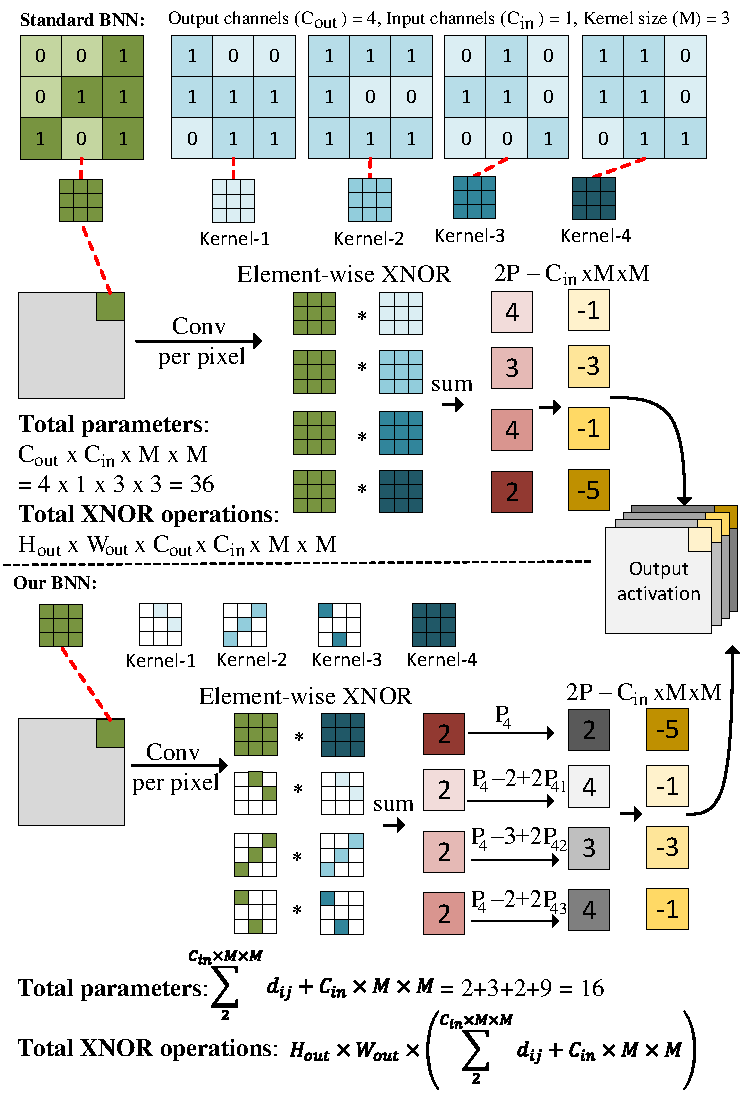
\includegraphics[width=1\textwidth]{images/images/MST_example.pdf}
	\end{center}
\end{minipage} 
\hfill
\begin{minipage}[t]{0.32\linewidth}
	\textbf{\color{\subheadercolor} HW architecture for a binary convolution}
	\begin{center}
		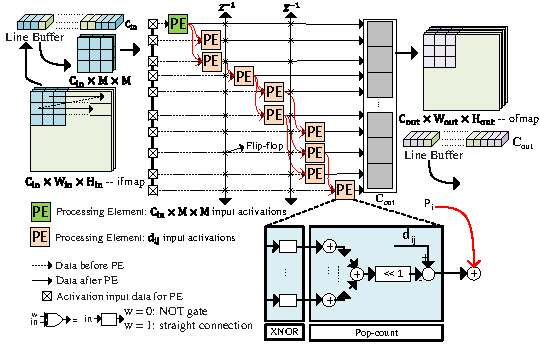
\includegraphics[width=1\textwidth]{images/images/MST_HW.pdf}
	\end{center}
	\textbf{\color{\subheadercolor} Computation process in HW architecture}
	\vspace{0.5em}
	\begin{itemize}
		{\scriptsize 
			\item \textbf{Loading input}: Image is loaded from DDR via DMA (Direct Memory Access) to BNN design. Line buffer with the size $C_{in}\times (W_{in}\times (M-1)+M)$ is valid when $C_{in}\times (W_{in}\times (M-2) + M - 1)$ is filled if the padding size = $1$, or fully filled if there is no padding.\\
			\item \textbf{Computation process}: The computation is in order following the MST. The output channel corresponding to the root vertex is calculated first with $C_{in}\times M\times \XNOR$ operations. From the next one, output of a vertex is calculated based on the previous output corresponding to the parent vertex and the output of a specific number of $\XNOR$ euqualing to the distance to the parent vertex.\\
			\item \textbf{Output storage}: The whole design is fully implemented; thus ofmap is delivered to the next layer without intermediate memory.
			\item \textbf{Performance}: Images are loaded to the design every clock cycle; thus throughput is not affected by the inrease of layers.}
			
	\end{itemize}
\end{minipage}
}
%
\headerbox{\bf\color{\headercolor} Binary Convolution}{name=dataset,column=1,row=0,span=3}{
    \begin{minipage}[t]{0.55\linewidth}
        %\textbf{\color{\subheadercolor}Dataset Statistics}
        BNNs binarizes parameters and activations using Eq. (\ref{eq:binary_function}). 
        \begin{equation}
        	\label{eq:binary_function} 
        	x^b=\Sign(x)=\begin{cases}
        		+1,  \text{ if } x \geq 0,\\
        		-1,  \text{ otherwise.}
        	\end{cases}
        \end{equation}
        
        Given a binary convolution, output of the channel ith can be computed using Eq. (\ref{eq:weight-reuse}).
        \begin{equation}
        	\label{eq:weight-reuse}
        	Y_i = (2\sum_{j=1}^{C_{in}MM}\XNOR(\mathcal{A}^b_{ij},\mathcal{W}^b_{ij}) - C_{in}\times M\times M) \odot \alpha,
        \end{equation}
        
        The same input activation is used to compute all output channels, while ($1 \XNOR x) + (0 \XNOR x)$ is always $1$. We can calculate the output channel $j^{th}$ as in Eq. (\ref{eq:outputchannel}).
        \begin{equation}
        	\label{eq:outputchannel}
        	Y_j = 2(P_i - d_{ij} + 2P_{ij})-C_{in}\times M\times M .
        \end{equation} 
       
        
        %\vspace{-0.5em}
        %\begin{center}
        %    \includegraphics[width=0.9\textwidth]{images/real_data_stats-crop.pdf}
        %\end{center}
        %\vspace{-1em}
        %\textbf{\color{\subheadercolor}Samples in Static Scenes With GT}
        %\vspace{-0.6em}
        %\begin{center}
        %    \includegraphics[width=0.78\textwidth]{images/static_samples-crop.pdf}
        %\end{center}
        %\vspace{-1em}
        %\textbf{\color{\subheadercolor}Samples in Dynamic Scenes Without GT}
        %\vspace{-0.7em}
        %\begin{center}
        %    \includegraphics[width=0.78\textwidth]{images/dynamic_nogt_samples-crop.pdf}
        %\end{center}
    \end{minipage}
    \hfill
    \begin{minipage}[t]{0.45\linewidth}
        \textbf{\color{\subheadercolor}Relation between two output channels in a binary convolution layer}

        %{\scriptsize Row 1: the selected image sequence.\\[-0.5em]
        %    Rows 2 and 3: two sample pairs with low-exposure and high-exposure reference frames, respectively.}
        %\vspace{-0.7em}
        \begin{center}
            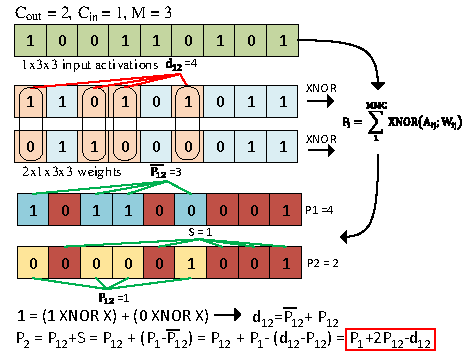
\includegraphics[width=1\textwidth]{images/images/weight-reuse_1.pdf}
        \end{center}
        %\vspace{-0.7em}
        %\begin{enumerate}
        %    \scriptsize
        %    \item The subject is asked to keep still for 2s, an HDR image is generated for this static frame
        %    \item The subject is asked to move back-and-forth (e.g., waving hands or walking)
        %    \item Select a sequence whose center frame was the static frame, and arrange it to be proper pairs 
        %\end{enumerate}
    \end{minipage}

}


\headerbox{\bf\color{\headercolor} Experiments \& Results}{name=results,column=4,span=2}{

\begin{minipage}[t]{0.48\linewidth}
	\textbf{\color{\subheadercolor}Effect of the number of centers}
	\begin{center}
		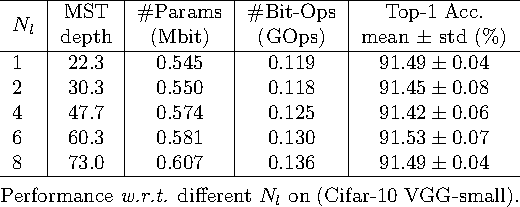
\includegraphics[width=1\textwidth]{images/images/center_table.pdf}
	\end{center}	
	\begin{center}
	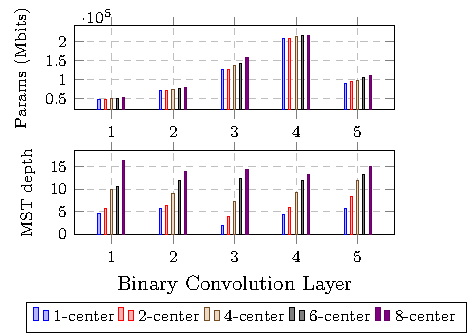
\includegraphics[width=1\textwidth]{images/images/center_chart.pdf}
	\end{center}	
\end{minipage}
\hfill
\begin{minipage}[t]{0.48\linewidth} 

	\textbf{\color{\subheadercolor}Effect of hyper-parameter $\lambda$}
	\vspace{-0.15em}
    \begin{center}
		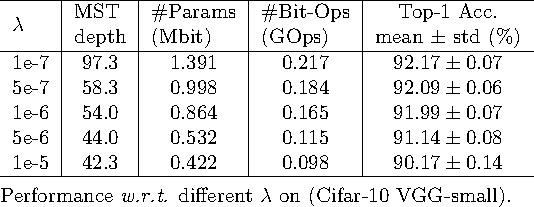
\includegraphics[width=1\textwidth]{images/images/lambda_table.pdf}
	\end{center} 
	%\begin{center}
		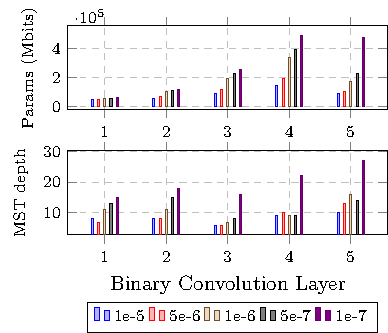
\includegraphics[width=0.9\textwidth]{images/images/lambda_chart.pdf}
	%\end{center} 
\end{minipage}
%-----------------------------

\begin{minipage}[t]{0.5\linewidth}
	\vspace{1em}
	\textbf{\color{\subheadercolor}Training comparison to SOTA}
	\vspace{0.5em}
	\begin{itemize}
		\scriptsize{
		\item \textbf{Ours 1}: After apply fine-tuning using the proposed learning optimization method.
		\item \textbf{Ours 2}: Apply only MST exploration and computation arrangement based on the MST for the inference without accuracy drop.}
	\end{itemize}
	\vspace{-0.2em}
	\begin{center}
		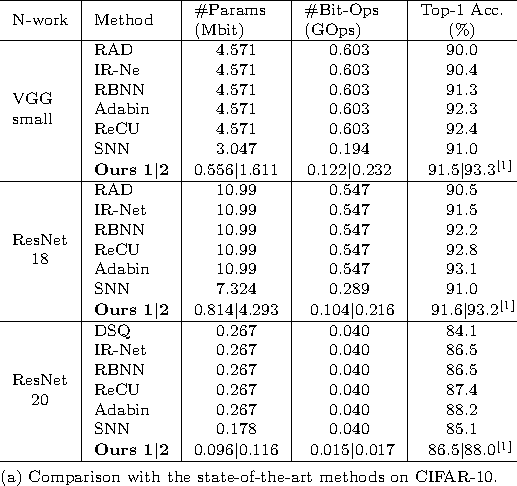
\includegraphics[width=1\textwidth]{images/images/Comparison_Cifar-10.pdf}
	\end{center} 
	\begin{center}
		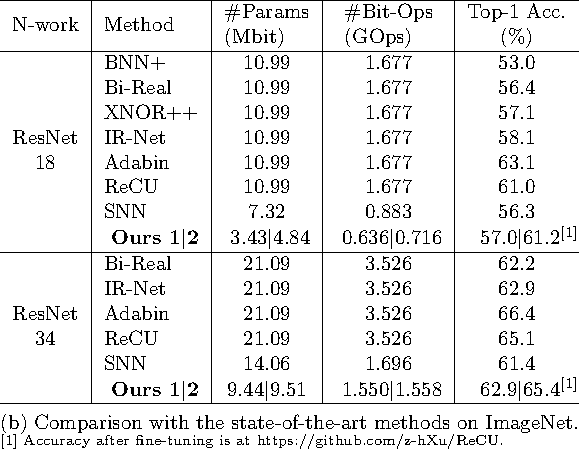
\includegraphics[width=1\textwidth]{images/images/ImageNet_comparison.pdf}
	\end{center} 
	
\end{minipage}
\hfill
 \begin{minipage}[t]{0.48\linewidth}
 \vspace{1em}
 \textbf{\color{\subheadercolor}Effect of hyper-parameter $\gamma$}
 \vspace{-0.5em}
 \begin{center}
 	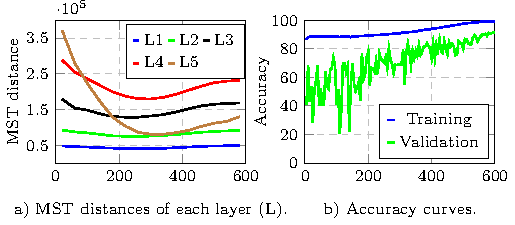
\includegraphics[width=1\textwidth]{images/images/accuracy.pdf}
 \end{center}
 \vspace{-0.5em}  
 \textbf{\color{\subheadercolor}HW comparison to SOTA designs}
 \begin{center}
 	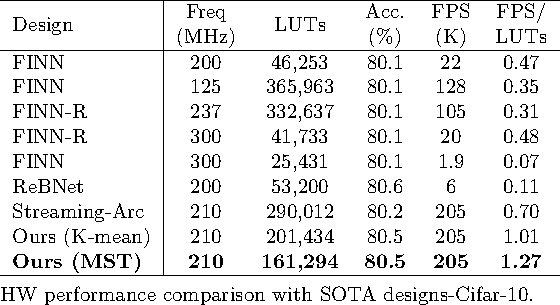
\includegraphics[width=1\textwidth]{images/images/HW_comparison.pdf}
 \end{center} 
 \vspace{-0.5em}
 \textbf{\color{\subheadercolor}References}
 \vspace{0.4em}
 \begin{enumerate}[leftmargin=*,label={[\arabic*]}]
 	\tiny
 	\item ReCU: Reviving the dead weights in binary neural networks, ICCV 2021
 	\item RAD: Regularizing activation distribution for training binarized deep networks, CVPR 2019
 	\item IR-Net: Forward and backward information retention for accurate binary neural networks, CVPR 2020
 	\item SNN: Sub-bit neural networks: Learning to compress and accelerate binary neural networks, ICCV 2021
 	\item Streaming-Arc: A deep learning accelerator based on a streaming architecture for binary neural networks, IEEE Access 2022
 	\item Finn: A framework for fast, scalable binarized neuralnetwork inference, ACM/SIGDA international symposium on FPGAs, 2017
 \end{enumerate}
 \vspace{0.5em}
 \textbf{\color{\subheadercolor}Future Research}
 \vspace{0.4em}
 \newline
 \tiny
 We have proposed a comprehensive compression method for BNNs from learning to accelerating with high throughput and resource efficiency purposes.
 In future work, to diversify the method's applications, we focus on improve the learning optimization that help the acceleration better compress.
 In terms of hardware implementation, architectures with limited number of processing elements would be considered to reduce the resources with acceptable throughput.
\end{minipage} 

}


\end{poster}
\end{document}
